\documentclass[10pt, twocolumn]{aastex62}
\newcommand{\vdag}{(v)^\dagger}
\newcommand\aastex{AAS\TeX}
\newcommand\latex{La\TeX}
\usepackage{amsmath}
\usepackage{physics}
\usepackage{hyperref}
\usepackage{natbib}
\usepackage{url}
\usepackage[T1]{fontenc}
\usepackage[english]{babel}
\usepackage[utf8]{inputenc}
\usepackage{layouts}
 \renewcommand{\familydefault}{\sfdefault}
\begin{document}

\title{Solving integrals by means of Guassian quadrature and Monte Carlo integration methods}

\author{Håkon Tansem}

\author{Nils-Ole Stutzer}

\author{Bernhard Nornes Lotsberg}

\begin{abstract}
	We have implemented, tested and compared four different numerical methods
	for solving integrals. The methods implemented were a brute force
	Gauss-Legendre quadrature, an improved Gauss-Laguerre quadrature as well as
	a brute force and an improved Monte Carlo integration method. These methods were
	tested on an integral computing the expectation value for the potential of
	two interacting electrons in a simplified helium atom with a known
	analytical solution. Our results indicate that for the integral, the relative
	error for the improved Gaussian quadrature method steadily decreases as the
	resolution of the computational grid increases. The brute force method on
	the other hand produces a relative error fluctuating unpredictably as the
	resolution of the grid increases making it inferior to the improved method
	when solving this integral. For the Monte Carlo methods we show that adapting the
	probability distribution to the given integral dramatically improves the
	variance, thereby gaining a significant increase in precision. The Monte
	Carlo methods were also calculated using parallelization indicating that the
	CPU time decreases proportionally to the amount of CPU threads used in the
	calculation. When taking the relative error into account our results
	indicate that for the integral, the improved Monte Carlo method is the
	preferred method of choice followed by the Gauss-Lagurre quadrature method. \\\\
	The source codes for this paper can be found at
	\href{https://github.com/bernharl/FYS4150-Project-3}{https://github.com/bernharl/FYS4150-Project-3}.  
	 
\end{abstract}

\section{Introduction} \label{sec:intro}
When solving problems in science and mathematics an ever recurring problem is to
solve integrals. Integrals are found in many problems in various fields such as
physics and economics. In this paper we consider ways of solving an example
of a six dimensional expectation value problem from quantum mechanics
in several different ways. We consider a brute force Gauss-Legendre quadrature,
an improved Gauss-Laguerre quadrature, a brute force monte carlo integration and
a monte carlo integration with importance sampling as shown by \cite{press:2007}
and \cite{jensen:2015}. The resulting integrals are compared to the
analytical solution and the run times are compared, in order to find which
method is most efficient.

In the theory section we present needed theory wich we discuss how to implement
in the method section. The results are presented in the results section and
discussed in the discussion section.

\section{Theory} \label{sec:theory}
\subsection{The integral}\label{subsec:integral}
Before stating the needed integration methods we present the integral to
integrate. Assuming the wave function of two electrons can be modelled as a
single-particle wave function in a hydrogen atom, the wave function of the $i$th
electon in the 1 $s$ state is given by 
\begin{align}
	\psi_{1,s}(\vec{r}_i) = e^{-\alpha r_i},
\end{align}
where the dimensionless position
\begin{align}
	\vec{r}_i = x_i \hat{e}_x + y_i\hat{e}_y + z_i\hat{e}_z
\end{align} 
with orthogonal unit vectors $\hat{e}_i$.

The distance from the origin is expressed as $r_i = \sqrt{x_i^2 + y_i^2 + z_i^2}$ and we let the parameter
$\alpha = 2$ corresponding to the charge of a helium $Z = 2$ nucleus. Then the ansatz
for the wave function for two electrons is given by the product of the two 1$s$
wave functions 
\begin{align}
	\Psi(\vec{r}_1, \vec{r}_2) = e^{-\alpha(r_1 + r_2)}.
\end{align}
We want to find the expectation value of the correlation energy between
electrons which repel each other by means of the Coulomb interaction as 
\begin{align}
\langle \frac{
1}{\vec{r}_1 - \vec{r}_2}\rangle = \int d\vec{r}_1d\vec{r}_2 e^{-2\alpha(r_1 + r_2)}\frac{1}{|\vec{r}_1 - \vec{r}_2|}.
\label{eq:integral}
\end{align}
This integral has an analytical solution $5\pi^2/16^2$, which we can compere to
the numerical results.
\subsection{Brute Force Gauss-Legendre Quadrature}\label{subsec:brute_force_gauss}
The following theory and derivations of the integration methods presented
follow closely \citep[Ch. 5.3]{jensen:2015}. 

The essence of Gaussian Quadrature (GQ) is to approximate an integral 
\begin{align}
	I = \int f(x) dx \approx \sum^N_{i = 1} \omega_i f(x_i),
	\label{eq:quadrature}
\end{align} 
for the weights $\omega_i$ and grid points $x_i$. The grid points and weights
are obtained through the zeros of othogonal polynomials. These polynomials are
orthogonal on some interval, for instance $[-1, 1]$ for Legendre polynomials.
Since we must find $N$ grid points and weigths, we must fit $2N$ parameters.
Therefore we must approximate the integrand $f(x)$ with a polynomial of degree
$2N-1$, i.e. $f(x) \approx P_{2N-1}(x)$. Then the integral 
\begin{align}
	I \approx \int P_{2N-1}(x)dx = \sum^{N-1}_{i=0}P_{2N-1}(x_i) \omega_i.
\end{align} 
GQ can integrate all polynomials of degree up to $2N-1$ exactly, we thus get
an equality when approximating the integral of $P_{2N-1}$. 

If we choose to expand the polynomial $P_{2N-1}$ in terms of the Legendre
polynomials $L_N$, we can through polynomial division write 
\begin{align}
	P_{2N-1} = L_N(x)P_{N-1}(x) + Q_{N-1}(x),
\end{align}
where $P_{N-1}$ and $Q_{N-1}$ are polynomials of degree $N-1$. We can thus write

\begin{align}
	I \approx \int^1_{-1} P_{2N-1}(x) dx &= \int^1_{-1} (L_N(x)P_{N-1}(x) + Q_{N-1}(x))dx \\
	&= \int^1_{-1}Q_{N-1}(x)dx,
\end{align}
where the last equallity is due to the orthogonallity between $L_N(x)$ and
$P_{N-1}(x)$. Furthermore, $P_{2N-1}(x_k) = Q_{N-1}(x_k)$ for the zeros $x_k$
($k = 0, 1, 2,\ldots, N-1$) of $L_N$, we can fully define the polynomial
$Q_{N-1}(x)$ and thus the integral. The polynomial $Q_{N-1}(x)$ can further be
expanded in terms of the Legendre basis 
\begin{align}
	Q_{N-1}(x) = \sum^{N-1}_{i=0} \alpha L_i(x).
	\label{eq:Qexpansion_of_x}
\end{align}
When integrating this we get
\begin{align}
	\int^1_{-1}Q_{N-1}(x)dx = \sum^{N-1}_{i=0} \alpha_i\int^1_{-1}L_0(x)L_i(x) dx = 2\alpha_0,
\end{align}
where we insert that the first Legendre polynomial is normalized to $L_0 = 1$
and utilize the orthogonality relation of the Legendre basis.

Since we know the value of $Q_{N-1}(x)$ at the zeros of $L_N(x)$, we can rewrite
(\ref{eq:Qexpansion_of_x})
\begin{align}
	Q_{N-1} (x_k)= \sum^{N-1}_{i=0} \alpha L_i(x_k).
	\label{eq:Qexpansion}
\end{align}
The resulting matrix $L_i(x_k) = L_{ik}$ has linearly independent columns due to
the Legendre polynomials being linearly independent as well. Therefore the
matrix $L_{ik}$ is orthogonal, i.e.
\begin{align}
	L^{-1}L = I.
\end{align}
We multiply both sides of (\ref{eq:Qexpansion}) by
$\sum^{N-1}_{i=0}L^{-1}_{ij}$, so that 
\begin{align}
	\alpha_k = \sum_{i=0}^{N-1} (L^{-1})_{ki}Q_{N-1}(x_i).
\end{align}
This result in addition to the approximation of the integral gives
\begin{align}
	I &\approx \int^1_{-1} P_{2N-1}(x)dx = \int^1_{-1} Q_{N-1}(x)dx = 2\alpha_0 \\
	&= 2 \sum^{N-1}_{i=0} (L^{-1})_{0i}P_{2N-1}(x_i).
	\label{eq:int_approx}
\end{align}
Here we can clearly see that the weights $\omega_i = 2(L^{-1})_{0i}$ and the
mesh points $x_i$ are the zeros of $L_N(x)$. Finding the weights is now simply a
matrix inversion problem and the mesh points can be found by for instance Newton's
method. Thus (\ref{eq:int_approx}) is on the same form as (\ref{eq:quadrature}),
yielding an approximation of $I$. When performing an integral with more general
limits $[a,b]$, one can now perform a simple change of variables $\tilde{x} =
\frac{b - a}{2}x + \frac{b + a}{2}$, to accomodate for this. Note that when
considering the Gauss-Legendre approach, and we integrate (\ref{eq:integral})
using cartesian coordinates, we must let the limits of all six cartesian
itegrals $a = -\lambda$ and $b = \lambda$ where $\lambda\to\infty$.

When integrating a six dimensional integral like the quantum mechanical problem
stated earlier, we can simply use Gauss-Legendre quadrature on all six integrals
in a brute force way. The integral becomes 
\begin{align}
	I &= \int d\vec{r}_1d\vec{r}_2 e^{-2\alpha(r_1 + r_2)}\frac{1}{|\vec{r}_1 - \vec{r}_2|} \\
	&\approx \sum_{i, j, k, l, m, n = 0}^{N-1} \omega_i \omega_j \omega_k \omega_l \omega_m \omega_n f,
\end{align} 
where $f = f(x_1^i, y_1^j, z_1^k, x_2^l, y_2^m, z_2^n)$ denotes the integrand
and each cartesian variable $x_i$ has the same weights $\omega$ due to identical
integration limits on the six integrals. 

\subsection{Improved Gaussian Quadrature}\label{subsec:improved_gauss}
The above mentioned Gauss Laguerre quadrature is in fact quite inaccurate in the
case of our integral. In order to improve on the method, one can use a different
orthogonal polynomial basis. In our case since we have an integral on the form
\begin{align}
	I = \int^\infty_0 f(x)dx = \int^\infty_0x^2e^{-x}g(x) dx
	\label{eq:laguerre_integral}
\end{align}
it is in fact more efficient to use Laguerre polynomials as opposed to
Legendre polynomials. Then when finding an approximation of the integral the
$x^2e^{-x}$ factor of the integrand is absorbed into the weights $\omega_i$,
making the weights more suitable for this specific integrand.
The derivation of the weights is however not shown here as it is completely
analogous to the derivation shown for the Gauss-Legendre quadrature.

In order to transorm our integrand to a form resembling
(\ref{eq:laguerre_integral}) we need to transform from cartesian to spherical
coordinates, i.e. $(x, y, z)\to(r, \theta, \phi)$ where $r\in[,\infty)$,
$\theta\in[0,\pi]$ and $\phi\in[0,2\pi]$. In spherical coordinates we get that the differential and the relative distance between the
electrons become 
\begin{align}
	d\vec{r}_1d\vec{r}_2 &= r_1^2r_2^2 dr_1dr_2\sin(\theta_1)\sin(\theta_2)d\theta_1d\theta_2d\phi_1d\phi_2\\
	|\vec{r}_1 - \vec{r}_2| &= \sqrt{r_1^2 + r_2^2 - 2r_1r_2cos(\beta)},
\end{align}
where $cos(\beta) = cos(\theta_1)\cos(\theta_2) +
\sin(\theta_1)\sin(\theta_2)\cos(\phi_1 - \phi_2)$. Next we introduce the change
of variables $u = \alpha r \implies du = \alpha dr$ so that the integral is on
the form
\begin{align}
	I = \frac{1}{32 \alpha^5} \int^\pi_0\int^{\pi}_0\int^{2\pi}_0\int^{2\pi}_0\int^\infty_0\int^\infty_0 fdu_1du_2d\theta_1d\theta_2d\phi_1d\phi_2,
	\label{eq:spherical_integral}
\end{align}
where $f = f(u_1, u_2, \theta_1, \theta_2, \phi_1, \phi_2) = \frac{\sin
	(\theta_1)\sin(\theta_2)u_1^2u_2^2e^{-(u_1+u_2)}}{\sqrt{u_1^2 + u_2^2 -
	2u_1u_2cos(\beta)}}$ is the new integrand. Now, for the radial part ($u_1$
	and $u_2$) a Gauss-Laguerre approach is used, while we use Gauss-Legendre
	quadrature for the angular part. 

\subsection{Brute Force Monte Carlo Integration}\label{subsec:brute_force_monte_carlo}
An integration method frequently used, especially when computing
multi-dimensional integrals as its error remains independent of the
dimensionality of the integral \citep[p. 343-344]{jensen:2015}, is the Monte Carlo integration. This integration method
approximates the integral with an expectation value. Consider for instance an
integral 
\begin{align}
	I &= \int^b_a f(x)dx = (b-a)\int^b_a\frac{f(x)}{b-a}dx \\	
	&= (b-a)\int^b_af(x)p(x)dx,
\end{align}
where we let $p(x) = \frac{1}{b-a}$ be the uniform probability density function
PDF for stochastic variables $x\in[a, b]$. Since we know that an expectation
value 
\begin{align}
	\langle f(x)\rangle = \int^b_a f(x)p(x)dx \approx \frac{1}{N}\sum_{i=0}^{N-1} f(x_i),
\end{align}
where we used that the expectation value of $f(x)$ is approximately the average
of the $f(x_i)$-s where the $x_i$-s are drawn from the distribution $p(x)$, for
large enough sample size $N$. 

Note that we implicitly performed a mapping in this case. Because uniform
distribution by default only returns values $y\in[0, 1]$, we change the variable
to $x = a + (b-a)y$ so as to draw values $x_i$ from a uniform distribution
between $a$ and $b$. 

The integral can thus be approximated by 
\begin{align}
	I \approx (b-a)\langle f(x) \rangle \approx \frac{b-a}{N}\sum^{N-1}_{i=0}f(x_i).
\end{align}
In order to get an estimate for the accuracy of the integration we can calculate
the variance defined as 
\begin{align}
	\sigma^2 = \frac{1}{N}\sum_{i=0}^{N-1} f^2(x_i) - \left(\frac{1}{N}\sum_{i=0}^{N-1}f(x_i)\right)^2 = \langle f^2\rangle - \langle f\rangle^2.
\end{align}
The variance for a multi-dimensionl case is computed ina completely analogous way.
As a Monte Carlo integration is a statistical experiment, the variance
$\sigma^2$ is a measure of the spread from the mean of the integral
approximation. We thus want to minimize this quatity.

When solving (\ref{eq:integral}) using cartesian coordinates, we use the same
integration limits as in the Gauss-Legendre quadrature. The we simply get a
six-dimensional expectation value so that 
\begin{align}
	I = (b-a)^6\langle f \rangle \approx \frac{(b-a)^6}{N}\sum^{N-1}_{i=0} f(x_1^i, y_1^i, z_1^i, x_2^i, y_2^i, z_2^i),
\end{align}
where the cartesian coordiantes $x^i$ are all drawn from a uniform distribution
for $x^i\in[-\lambda, \lambda]$. The variance is calculated completely analogously
to the one-dimensional case. 

\subsection{Improved Monte Carlo Integration}\label{subsec:improved_monte_carlo}
One way to improve the Monte Carlo Integration shown in the previous subsection,
i.e. to reduce its variance, is to use a different PDF, that fits the shape of
the integrand better, to draw the samples from.

If we consider the quantum mechanical integral in spherical coordinates, as
shown previously, we recognize the $e^{-u}$ factors as an exponential
distribution. Thus we let $p(y) = e^{-y}$ denote the exponential distribution.
Using conservation of probability under change of variable, we set $p(y)dy =
\exp(-y)dy = p(x)dx = dx$ for the uniform PDF $p(x)$ with $x\in[0,1]$. If we
integrate this cumulative distribution we find 
\begin{align}
	x(y) = \int^y_0 \exp(-\xi)d\xi = 1 - \exp(-y),
\end{align} 
which we can invert to get the mapping $y(x) = -\ln(1-x)$ from the uniform to
the exponential PDF. Now $u = y\in[0\infty)$ is used for the radial distance. We
can now absorb the exponential part of the integral into the expectation value
so that 
\begin{align}
	I &= \int^\infty_0 f(u)du = \int_0^\infty \frac{f(u)}{p(u)}p(u)du \\
	&= \int^1_0 g(u(x))dx \approx \frac{1}{N}\sum_{i=0}^{N-1} g(u(x_i), 
\end{align}
where we use that $p(u) = \exp(-u)$ and $p(u)du = dx$ to change variables.
The samples $u(x_i)$ are now drawn from the exponential distribution $p(u)$.
This is what is called importance sampling, which results in a lower variance
than using the brute force Monte Carlo integration, because we sample
from a distribution which fits the shape of the integrand better. 

Note that the integral we want to estimate in spherical coordinates
only has limits $[0, \infty)$ for the two radial coordiantes $u_1$ and $u_2$. We
must thus sample from the uniform distribution for the angular integrals, as the
angles exist within the finite limits $[0,\pi]$ and $[0, 2\pi]$, while the radial
integral should utilize importance sampling from the exponential distribution.

The final integral looks as follows
\begin{align}
	I \approx \frac{1}{N}\frac{\pi^4}{8\alpha^5}\sum^{N-1}_{i=0}\frac{\sin
	(\theta_1^i)\sin(\theta_2^i)(u_1^i)^2(u_2^i)^2}{\sqrt{(u_1^i)^2 + (u_2^i)^2 - 2u_1^iu_2^icos(\beta_i)}},
\end{align}
where the index $i$ simply represents that the corresponding samples are drawn
from their corresponding PDFs.
\section{Method} \label{sec:method}
When approximating the integrals, one may encounter singularities in the
integrand when $|\vec{r}_1 - \vec{r}_2|$ becomes too small, which is due to the
discretization. In order to handle these singularies we simply let the integrand
$f=0$ when this happens. 

Next when implementing the two GQ integrators, the integration sum approximating
the six-dimensional integral are calculated in a sixfold loop. When
calculating the integration weights and grid points we use the algorithms
presented in (\cite{press:2007}) (implemented in the \texttt{weights.cpp}-file).
In the brute force cartesian GQ approach as well as the angular integrals in the
improved GQ we compute the weights and meshpoints using the provided
\texttt{gauleg}-function, since the integration limits are finite, while the weights
and mesh points of the radial integral are produced using the provided
\texttt{gauss\_laguerre}-function. The integrals are calulated with the two GQ
methods for different grid sizes $N$ and then compared. In order to produce a
satisfactory result using the brute force Gauss-Legendre quadrature we tried
different grid sizes $N$ and approximation of infinity $\lambda$.

When implementing the Monte Carlo integrations, we produce the needed
psuedo-random numbers using a Mersenne-Twister algorithm, as it has a
sufficiently large period. Furthermore the mapping from the uniform PDF with
$x\in[0,1]$ to the uniform PDF with $x\in[a,b]$ and the exponential
distributions are done implicitly inside the C++ \texttt{random}-packages used.
The Monte Carlo integrals are computed for different sample sizes $N$,
different degrees of parallelization using OpenMP and different compiler flags,
for comparison. 

\section{Results} \label{sec:results}
The results were produced running on a MacBook Pro (macOS Mojave 10.14.6) with
8GB RAM using a dual core Intel Core i5-7360U $2.3$GHz CPU with four threads.
The program was compiled using OpenMP for the parallelization with the gcc
compiler version (Homebrew GCC $9.2.0\_1$) $9.2.0$.\\\\ 
For the results listed below we found that $\lambda = 1.5$ was a sufficient
approximation for infinity when using grid sizes $N\sim20$ to $N\sim 30$ when
using brute force Gaussian quadrature as described in section
\ref{subsec:brute_force_gauss}. This choice for $\lambda$ remained the same when
calculating the brute force Monte Carlo method as described in section
\ref{subsec:brute_force_monte_carlo}. When calculating the integral, the
relative error was calculated for the integral given by (\ref{eq:integral}) using
the brute force method, as describred in section
\ref{subsec:brute_force_gauss}. The relative error was also calculated for the
integral in spherical coordinates given by (\ref{eq:spherical_integral}) using
the improved method, as described in section \ref{subsec:improved_gauss}. These
results are shown in Figure \ref{fig:relerrquad}. In the figure a line is drawn
to illustrate when the method achieves three digit precision. The CPU time for
the improved Gaussian quadrature method with grid resolution $N=30$ was
measured to be approximately $51000$ms\\

\begin{figure}[h]
	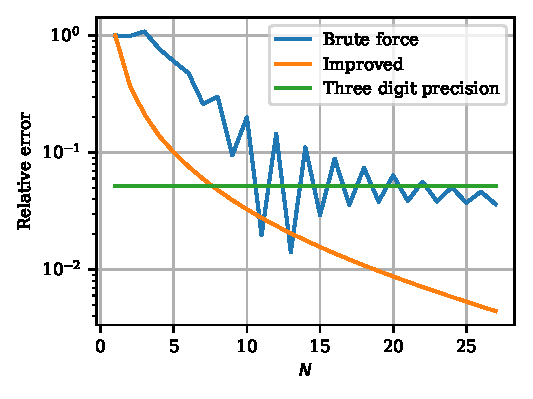
\includegraphics{{Figures/exercise_a_b}.pdf}
	\caption{Figure showing the relative error for the brute force Gaussian quadrature and the improved Gaussian quadrature methods, described in section \ref{subsec:brute_force_gauss} and \ref{subsec:improved_gauss} respectively, as a function of grid resolution $N$. A line is drawn to illustrate when the integral reaches three digit precision.}
	\label{fig:relerrquad}
\end{figure}
The relative error was also compared for both the brute force and the improved
Monte Carlo methods described in section
\ref{subsec:brute_force_monte_carlo} and \ref{subsec:improved_monte_carlo}
respectively. This is shown in Figure \ref{fig:rellerrcarlo}. For the same
calculations using both Monte Carlo methods, the variance was also plotted. This
is result is illustrated in Figure \ref{fig:variancecarlo}. 
\begin{figure}[h]
	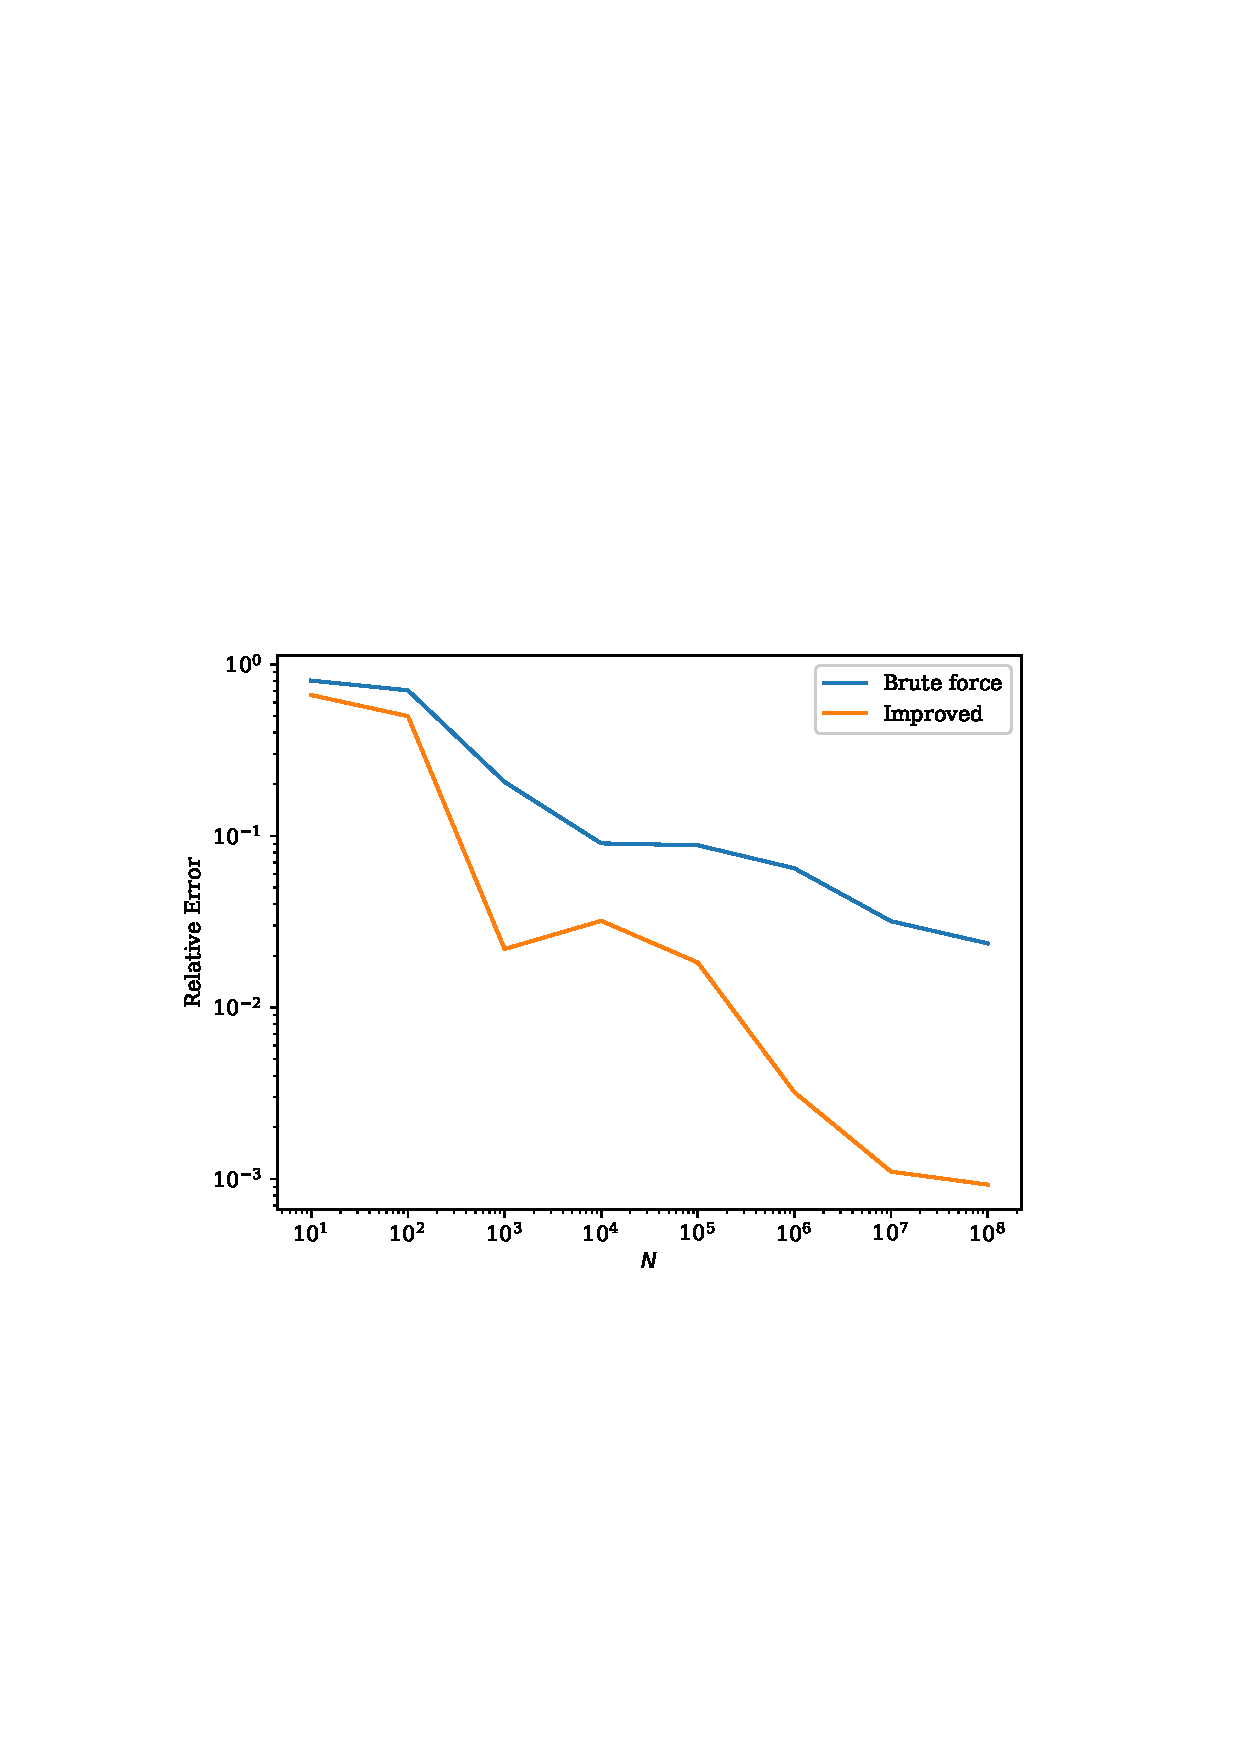
\includegraphics{{Figures/error_monte_carlo}.pdf}
	\caption{Figure showing the relative error for the brute force and the improved Monte Carlo methods, described in section \ref{subsec:brute_force_monte_carlo} and \ref{subsec:improved_monte_carlo} respectively, as a function of the sample size $N$.}
	\label{fig:rellerrcarlo}
\end{figure}

\begin{figure}[h]
	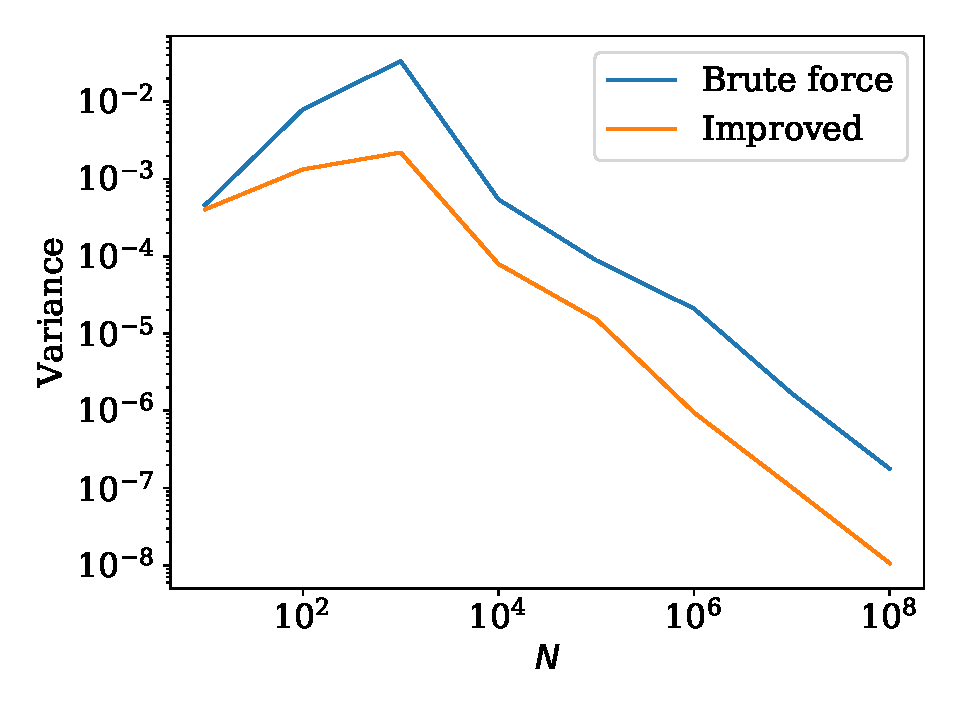
\includegraphics{{Figures/variance_monte_carlo}.pdf}
	\caption{Figure showing the variance for the brute force and the improved Monte Carlo methods, as described in section \ref{subsec:brute_force_monte_carlo} and \ref{subsec:improved_monte_carlo} respectively, as a function of the sample size $N$.}
	\label{fig:variancecarlo}
\end{figure}
The CPU time for both the brute force and the improved Monte Carlo methods were
calculated using no parallelization and parallelization with two threads. This
is shown in Figure \ref{fig:CPUcarlo}. The three different compiler flags -O1,
-O2 and -O3 were also compared to study their impact on the CPU time, which is
shown in Figure \ref{fig:CPUcarloflag}. This result was produced using no parallelization.
\begin{figure}[h]
	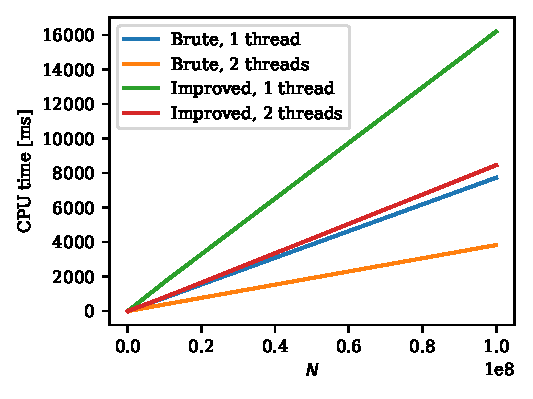
\includegraphics{{Figures/cpu_time_monte_carlo}.pdf}
	\caption{Figure showing the CPU time for the brute force and the improved Monte Carlo methods, described in section \ref{subsec:brute_force_monte_carlo} and \ref{subsec:improved_monte_carlo} respectively, as a function of the sample size $N$. For both methods the CPU time was compared both unparallelized and parallelized with two threads.}
	\label{fig:CPUcarlo}
\end{figure}

\begin{figure}[h]
	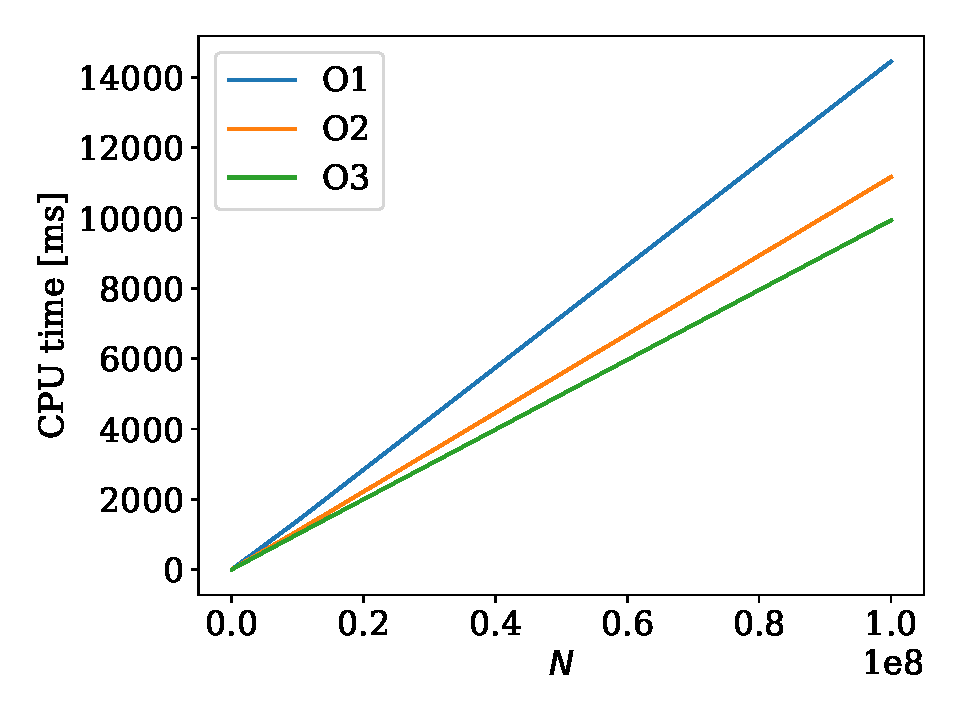
\includegraphics{{Figures/cpu_time_compilerflag}.pdf}
	\caption{Figure showing showing the CPU time for the improved Monte Carlo method, described in section \ref{subsec:improved_monte_carlo}, as a function of the sample size $N$ using the different compiler flags -O1, -O2 and -O3. These results were produced using no parallelization.}
	\label{fig:CPUcarloflag}
\end{figure}
\newpage
\section{Discussion} \label{sec:discussion}
When computing the integral (\ref{eq:integral}) using brute force Gaussian
quadrature, as mentioned in the section \ref{sec:results}, when
using a grid size of $N\sim20$ to $N\sim30$, we found that $\lambda = 1.5$ was a
sufficient approximation for infinity. This achieved a three digit
precision. However, one can in Figure \ref{fig:relerrquad} see that the relative
error of the Gauss-Legendre quadrature varies rapidly over the grid size $N$.
Thus, the brute force approach yields an unsatisfactory precision as it behaves unpredictably. Therewhile, the relative
error of the improved Gaussian quadrature decreases for increasing grid size $N$. Thus
the improved Gauss-Laguerre quadrature method provides a far more predictable
decrease in the relative error, making it the Gaussian quadrature of choice for
the problem at hand. The differences between these two methods are consistant
with the theory, as the Gauss-Laguerre quadrature constructs more suitable weights
fitting the integrand better. Also we need to approximate infinity when
computing (\ref{eq:integral}) in cartesian coordiantes using Gauss-Legendre
quadrature, while the Gauss-Laguerre quadrature using spherical coordiantes
absorbs the infinity term in the weights, effectively circumventing this
potential source of error of an insufficient infinity approximation.\\\\\indent


When comparing the relative error for the brute force and improved Monte Carlo
methods, our results, as shown in Figure \ref{fig:rellerrcarlo}, indicate that
the improved method reaches a significantly higher precision for higher sample
sizes $N$. This shows that when we draw from a probability distribution suited
to the integrand our results improve. This can also be seen by studying the
variance for the brute force and improved methods, as shown in Figure
\ref{fig:variancecarlo}. Here we see that the variance drops a lot faster for
the improved method and stays approximately an order of magnitude lower than the
variance for the brute force method.\\\indent 
When comparing the CPU time for the improved Gaussian quadrature method with
grid resolution $N=30$ to the CPU time for the improved Monte Carlo method with
sample size $N=10^8$, both unparallelized, one can see that the CPU time for the
improved Monte Carlo method is significantly better. If we compare the relative
error one can also see, from figures \ref{fig:relerrquad} and
\ref{fig:rellerrcarlo}, that the relative error for the improved Monte Carlo
method is a lot smaller. This indicates that the improved Monte Carlo method
provides a better accuracy for a shorter CPU time. It is also worth noting that
the results presented originate from a single run of the program. CPU time can
be sensitive to background processes running on the processor. This can cause
the results to vary slightly for different runs. A further improvement would be
to take the average over multiple runs. Another source for inaccuracy is the
approximation of infinity as $\lambda = 1.5$\\\\\indent

The parallelization provided a significant improvement to the CPU time for the
brute force and improved Monte Carlo methods. From Figure \ref{fig:CPUcarlo} one
can see that the parallelization with two threads approximately halves the CPU
time compared to doing the same calculation with one thread. From the same
figure, one can also see that the CPU time for the brute force method is
lower than the CPU time for the improved method. This shows that allthough increasing
precision, drawing from an exponential distribution comes with a drawback in
form of calculations taking longer time. This may be due to the logarithm
present in the mapping from the uniform distribution to the exponential
distribution, shown in section \ref{subsec:improved_monte_carlo}.\\

When studying the solution for the improved Monte Carlo method using no
parallelization and different compiler flags, our results indicated that the
flags had a low impact on the CPU time. This is shown in Figure
\ref{fig:CPUcarloflag}. In our implementation of the methods, we included an
if-statement to set $f=0$ if $|\vec{r}_1 - \vec{r}_2| = 0$ to avoid divison by
zero as described in section \ref{sec:method}. For the compiler flags to be able
to optimize the code, the code should be predictable. If-statements make the code
unpredictable in the sense that there is no way to predict when the condition
occurs. This makes it hard for the compiler to vectorize the loops. A further improvement would be to rewrite the integral given by
\ref{eq:integral} on a form that does not contain singularities both to improve
CPU time when using compiler flags as well as excluding potential errors from
setting $f=0$.



\section{Conclusion} \label{sec:conclusion}
We have implemented four different numerical integration methods to find the
expectation value of the potential of two interacting electrons in a simplfied
helium atom model. For the brute force Gauss-Legendre method in cartesian
coordianes, the relative error was found to fluctuate rapidly over increasing
grid size $N$. Therewhile the improved Gauss-Laguerre approach in spherical
coordinates provided a relative error steadily decreasing for increasing $N$,
rendering it the GQ of choice for the problem at hand. When Comparing the brute
force and improved Monte Carlo methods, we found that the improved Monte Carlo
method had a longer CPU time, however a the variance remained approximately an
order of magnitude lower than the brute force method throghout the calculations.
When comparing the improved GQ and Monte Carlo integration with the highest grid
and sample size tested, we found the Monte Carlo integration to provide the best
accuracy as well as having a significantly shorter CPU time.

When comparing the run time of the brute force and improved Monte Carlo
integrations for different sample sizes and different degrees of
parallelization, we found that the improved Monte Carlo method in general had a
longer CPU time than the brute force method. However, a notable speed up was
noticed when the method was parallelized using one and two threads.

Last we tested the CPU time of the improved Monte Carlo method with different
compiler flags without parallelization, for different grid sizes. We found
all three comiler flags to provide about the same CPU time, probably due to the
if-statement in the integrand preventing efficient vectorization.

In order to improve our results one could rewrite the integrand in a more
convecnients manner, so as to circumvent singularities. Also one could run the
Monte Carlo integrals and measure the CPU time several times for each sample size
$N$ and take the mean to get a more accurate results.

%\printinunitsof{in}\prntlen{\textwidth}
\nocite{jensen:2019}
\bibliographystyle{aasjournal}
\bibliography{ref}  

\end{document}

